\chapter{Methodology}\label{chapter:Methodology}

% \indent Citations should be included as \cite{Chen}, or \cite{Kondoz,atal} if there are more than one references to cite.

In TDLGC, the recommendation process is split into two phases:
\begin{itemize}
    \item First step is User-based rating prediction, where user's community and similarity matrices are used inorder to predict user-based ratings\cite*{9775081}.
    \item Second step is Food-based rating prediction, where food items are grouped into several clusters using a deep-learning based clustering algorithm\cite*{9775081, oulu_tdlgc} from which ratings on unseen foods are predicted.
\end{itemize}
Following these two steps, the Top-N foods are recommended\cite*{9775081} to the user.
\\
Fig 2.1\cite*{9775081, oulu_tdlgc} shows the model's conceptual framework, showcasing two distince phases: User-based rating prediction and Food-based rating prediction\cite*{9775081}. In the first phase, the model leverages user ratings along with the follower-following network inorder to generate user-user similarity matrix\cite*{9775081, oulu_tdlgc} and a trust network. Then, a graph clustering algorithm\cite*{ZHAO2021358} is used to group the users into different communities. Finally, it predicts the ratings of unseen foods for each user based on their cluster, similarity, and trust information. In the second phase, the model uses deep learning techniques to embed food ingredients into a latent space. Then, it calculates the similarity between different foods based on their embeddings. Finally, ratings on unseen foods for each user is predicted based on food similarity and historical ratings. After the two phases, the model combines the user-based and food-based rating predictions to generate a Top-N food recommendation list for each use.

\begin{figure}[htp]
    \centering
    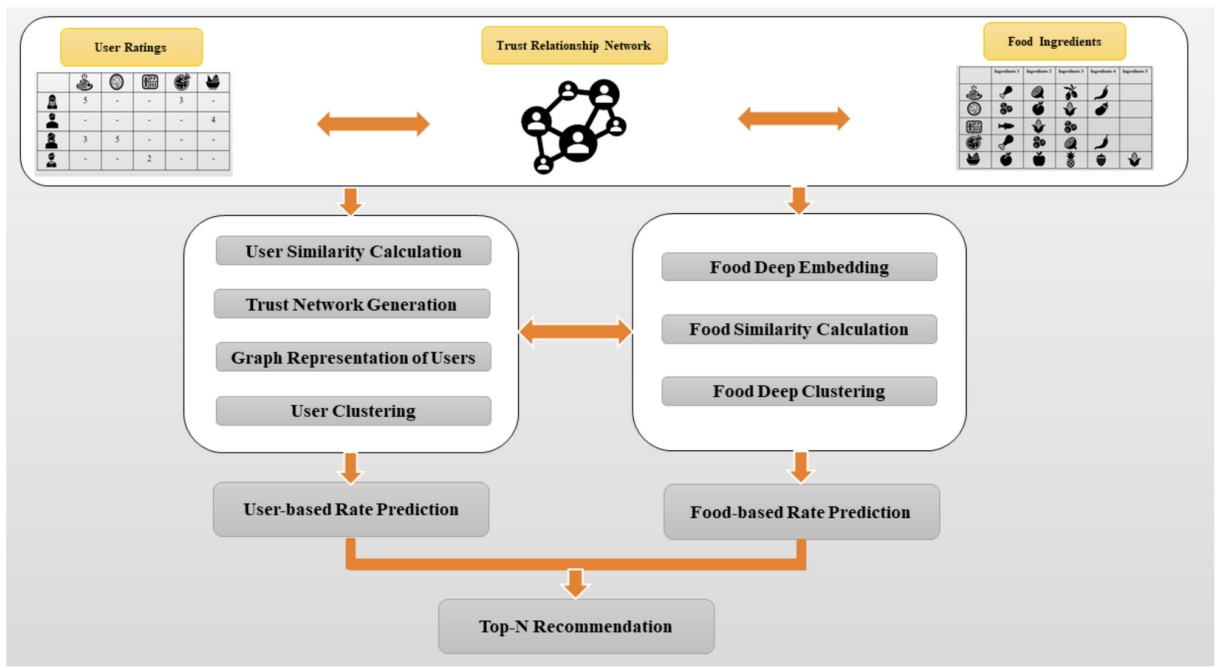
\includegraphics[width=12cm]{fig1_model_conceptual_framework.jpg}
    \caption{Conceptual framework of the model}
    \label{fig:framework}
\end{figure}

\section{User Based Rating Prediction}
\subsection{User Similarity Calculation}
Similarity measure between users is calculated using cosine similarity formula, which also takes into account ratings and time stamps of the user\cite*{9775081}.
\begin{equation*}
    sim\left({u_{i},u_{j}}\right)=\frac {a}{bc}, \tag{1}
\end{equation*}
where values of a, b, and c are found using the given formulae\cite*{9775081, oulu_tdlgc}:
\begin{align*}
    \begin{cases}
        \displaystyle a=\sum \nolimits _{k\in A_{u_{i},u_{j}}} \left({\left({r_{k}\left({u_{i}}\right)-\bar {r}\left({u_{i}}\right)}\right). \left({r_{k}\left({u_{j}}\right)}\right.}\right.
        \\
            \displaystyle \left.{\left.{\qquad \qquad -\bar {r}\left({u_{j}}\right)}\right)TW_{\left({u_{i},u_{j},k}\right)}}\right),
        \\
        \displaystyle b=\sqrt {\sum \nolimits _{k\in A_{u_{i},u_{j}}}^{}\left({\left({r_{k}\left({u_{i}}\right)-\bar {r}\left({u_{i}}\right)}\right)^{2}.TW_{\left({u_{i},u_{j},k}\right)}}\right)},
        \\[0.5pc]
        \displaystyle c=\sqrt {\sum \nolimits _{k\in A_{u_{i},u_{j}}}^{}\left({\left({r_{k}\left({u_{j}}\right)-\bar {r}\left({u_{j}}\right)}\right)^{2}.TW_{\left({u_{i},u_{j},k}\right)}}\right)}.
    \end{cases}
\end{align*}
Here, $TW_{(u_{i}, u_{j}, k)}$ represents the cumulative weights assigned to ratings of users $u_i$ and $u_j$ for food $f_k$ after factoring in time stamps of the ratings\cite*{9775081}. This weight is calculated as given in the below formula\cite*{9775081}:
\begin{equation*}
    {TW}_{\left({u_{i},u_{j},k}\right)}=e^{-\lambda \left({TP-t\left({u_{i},k}\right)}\right)}+e^{-\lambda \left({TP-t\left({u_{j},k}\right) }\right)} \tag{2}
\end{equation*}
$\lambda$ is a parameter which is controlled by the user in order to adjust the influence of time factor in calculating accumulative weight. TP indicates maximum Time Period.

\subsection{Generate Trust Network}
Trust network is a graph that represents the trust relationship among users. Some studies have shown that users who trust each other, will show profiles with similar ratings\cite*{MORADI2015462}. The assumption is made that if user $u_i$ follows user $u_j$, then there exists a trust relationship between them, or simply, user $u_i$ trusts user $u_j$. Trust network\cite*{9775081, oulu_tdlgc} is an unweighted and undirected graph TrustG(U, Tr), where U represents the set of users and Tr represents the collection of edges between users.
\\
\indent The Trust network can also be represented in the form of a weighted graph where edge weight between user $u_i$ and user $u_j$ is set to 1 if $u_i$ trusts $u_j$, else it is set to 0.

\subsection{Graph Representation of Users}
User set U is mapped onto a weighted graph G(U,E,W)\cite*{9775081, oulu_tdlgc}, where E represents set of edges linking users and W represents calculated similarities between different users in U. To calculate the edge weights between users, a combination of Pearson correlation coefficient and the trust network previously obtained is utilized\cite*{9775081}, as given in the below formula:
\begin{equation*} w(u_{i},u_{j})=\alpha.Tr\left({u_{i},u_{j}}\right)+\left({1-\alpha }\right).sim\left({u_{i},u_{j}}\right). \tag{3}\end{equation*}
where Tr($u_i$,$u_j$) denotes the trust score between users $u_i$ and $u_j$.
$\alpha$ is the control parameter that adjusts contributions of trust Tr($u_i$,$u_j$) and similarity sim($u_i$,$u_j$) values.

\subsection{User Clustering}
User clustering is a technique used to group users with similar preferences in recommender systems. A graph clustering algorithm based on graph compression\cite*{ZHAO2021358} to cluster users in a large and sparse user-food rating matrix. Nodes with high similarity are iteratively merged, and edge weights are updated according to node density and influence.
\\
\indent User clustering improves perfomance of user-based rating prediction by selecting more relevant neighbors for target user.

\subsection{User-based Rating Prediction}
Prediction for ratings of food $f_k$ based on user $u_i$ is calculated as given below\cite*{9775081}:
\begin{align*} p_{k}^{u-based}\left({u_{i}}\right)\!=\!\bar {r}\left({u_{i}}\right)+\frac {\sum _{u_{j}\in C_{i}}{w(u_{i},u_{j}).\left({r_{k}\left({u_{j}}\right)\!-\!\bar {r}\left({u_{j}}\right)}\right)}}{\sum _{u_{j}\in C_{i}}\left |{w_{(}u_{i},u_{j})}\right |}. \\\tag{4}\end{align*}
where w($u_i$, $u_j$) indicates weights between users $u_i$ and $u_j$. $C_i$ represents community to which user $u_i$ belongs to.
\\
Fig 2.2\cite*{9775081} shows how user-based rating prediction is being done for a sample dataset with nine users\cite*{9775081}. User-food matrix containing rating for food given by user is used to find similarity between users. This, along with the trust network between users is used to build a graph representation of the users using which users are clustered. This is used to predict ratings of previously unseen food item with respect to each user.
\begin{figure}[htp]
    \centering
    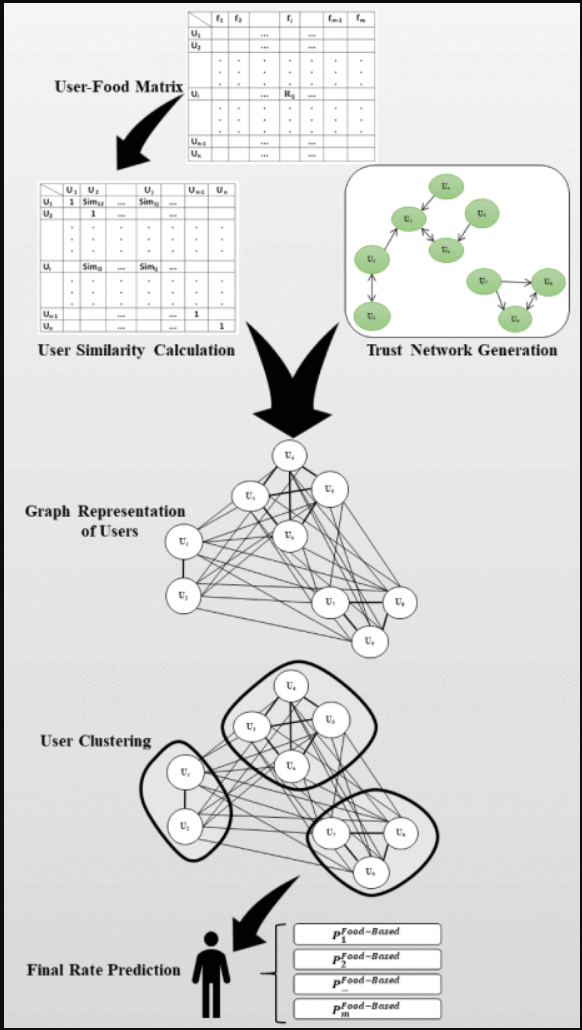
\includegraphics[scale=0.80]{overall_schema_user_based_rating_prediction.png}
    \caption{User-based rating prediction model for sample dataset with nine users}
    \label{fig:User-based rating prediction model}
\end{figure}


\section{Food Based Rating Prediction}
\subsection{Food Deep Embedding}
Food clustering based on ingredients is performed by utilizing the Bidirectional Encoder Representation from Transformer - Large (BERT-Large)\cite*{devlin2019bert}. It creates contextualized embeddings for foods. Inorder to apply Natural Langiage Processing(NLP) to food clustering, each food $f_i$ is considered as a sentence, with its ingredients $I_i$ as words\cite*{9775081, oulu_tdlgc} of the sentence.
\\
\indent Fig 2.3\cite*{9775081, oulu_tdlgc} shows how BERT is being used for food-based deep embedding\cite*{9775081}. To use Natural Language Processing (NLP) techniques for food clustering, each food $f_i$ is treated like a sentence, while its ingredients $I_i=\{ing_{\sigma(1)},ing_{\sigma(2)},ing_{\sigma(3)},\ldots,ing_{\sigma(k_i)}\}$ are treated as words in that sentence\cite*{9775081, oulu_tdlgc}. Feature extraction procedure takes the sentences(i.e. foods) and tokens(i.e. ingredients) as inputs, and generates an output JSON file - which contains simulated embeddings from different layers of BERT\cite*{9775081,devlin2019bert}. The embeddings are essentially representations of tokens as N-dimensional vectors, helping in capturing the context in which they appear.
\\
\indent The final step here invloves calculating average of all token representations within the sentence inorder to produce a contextualized representation\cite*{9775081, oulu_tdlgc}.
\begin{figure}[htp]
    \centering
    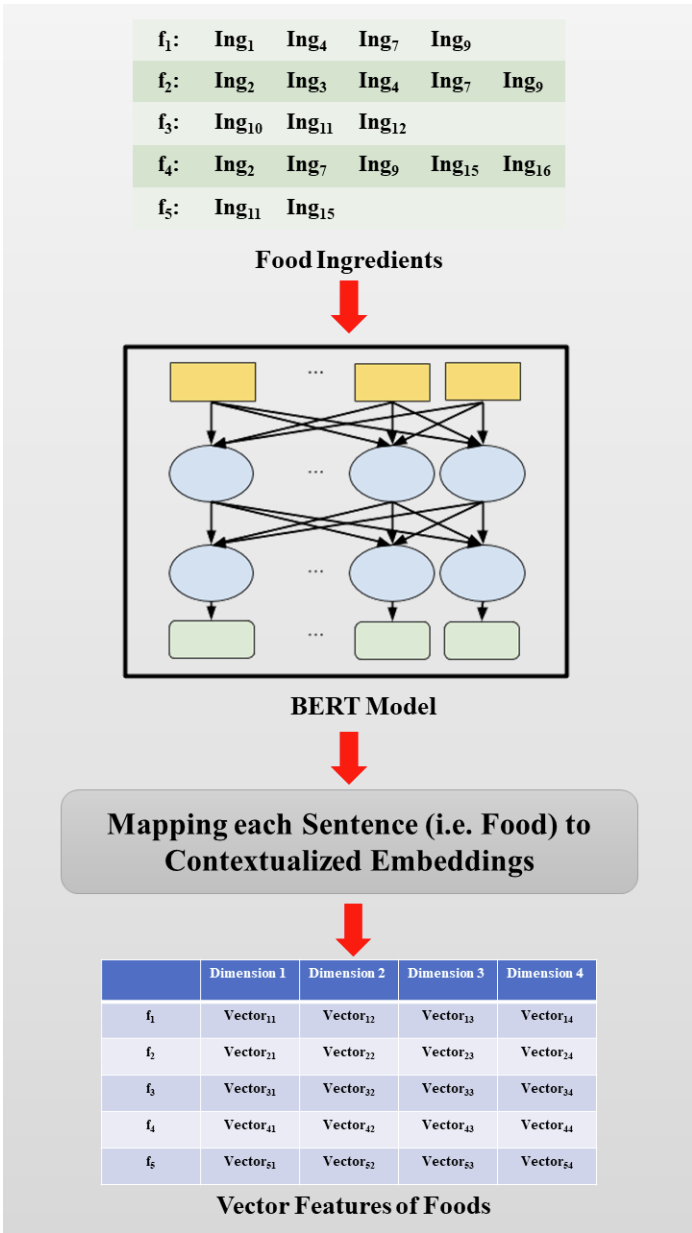
\includegraphics[scale=0.80]{overview_of_bert_based_food_embedding_method.png}
    \caption{Overview of BERT-based food embedding method}
    \label{fig:BERT-based food embedding}
\end{figure}

\subsection{Food Similarity Calculation}
By utilizing contextualized embeddings from previous step, ingredients present in a food can be identified. Similar food items are in close proximity to each other in the vector space and they are assumed to share some ingredients\cite*{9775081, oulu_tdlgc}. Euclidean distance formula is used in order to evaluate proximity between vectors of foods $f_i$ and $f_j$.
\\
\indent Let $f_i$ = \{$f_{i1}$, $f_{i2}$, $f_{i3}$, ... $f_{iL}$\} and $f_j$ = \{$f_{j1}$, $f_{j2}$, $f_{j3}$, ... $f_{jL}$\} be contextualized representation vector of food $f_i$ and $f_j$, respectively\cite*{9775081}. Similarity between $f_i$ and $f_j$ is calculated using Eucledian distance formula given as\cite*{9775081, oulu_tdlgc}:
\begin{equation*} Sim\left({f_{i},f_{j}}\right)=1-\left({\sqrt {\sum _{l=1}^{L}\left({f_{il}-f_{jl}}\right)^{2}}}\right). \tag{5}\end{equation*}
where $f_{il}$ denotes l - th dimension of the contextualized representations vector of the food $f_i$.

\subsection{Food Clustering}
This step is done to group foods based on their ingredients, and overcome the data sparsity and cold start problems of collaborative filtering-based food recommender systems. It reduces distance between similar embedding vectors.
\\
\indent Deep Embedded Clustering technique is used to reduce distance between similar embedding vectors in embedding space\cite*{DBLP:journals/corr/XieGF15}. AutoEncoders and Kullback-Leiber divergence is used here to decrease the data dimensions and enhance the embedding vector representation\cite*{9775081, oulu_tdlgc}.

\subsection{Food-based Rating Prediction}
For food-based rating prediction, rating of food $f_i$ for user $u$ is calculated as:
\begin{equation*} p_{i}^{f-based}\left({u}\right)={\bar {r}}_{i}+\frac {\sum _{j\in C_{f_{i}}}{sim\left({f_{i},f_{j}}\right).\left({r_{j}\left({u}\right)-{\bar {r}}_{j}}\right)}}{\sum _{j\in C_{f_{i}}}\left |{sim\left({i,j}\right)}\right |}.\quad \tag{6}\end{equation*}
Fig 2.4\cite*{9775081, oulu_tdlgc} shows food-based rating prediction for a sample dataset having seven different food items\cite*{9775081, oulu_tdlgc}. User-food matrix and the food ingredient matrix is utilized along with BERT to perform food deep embedding. Proximity of food items in vector space is used as a factor in measuring similarity between them, and Eucledian distance formula is used to calculate this similarity. Deep Embedded Clustering technique is used to cluster the food items. Based on similarities between different foods and their previous ratings given by users, ratings of unseen foods are predicted.

\begin{figure}[htp]
    \centering
    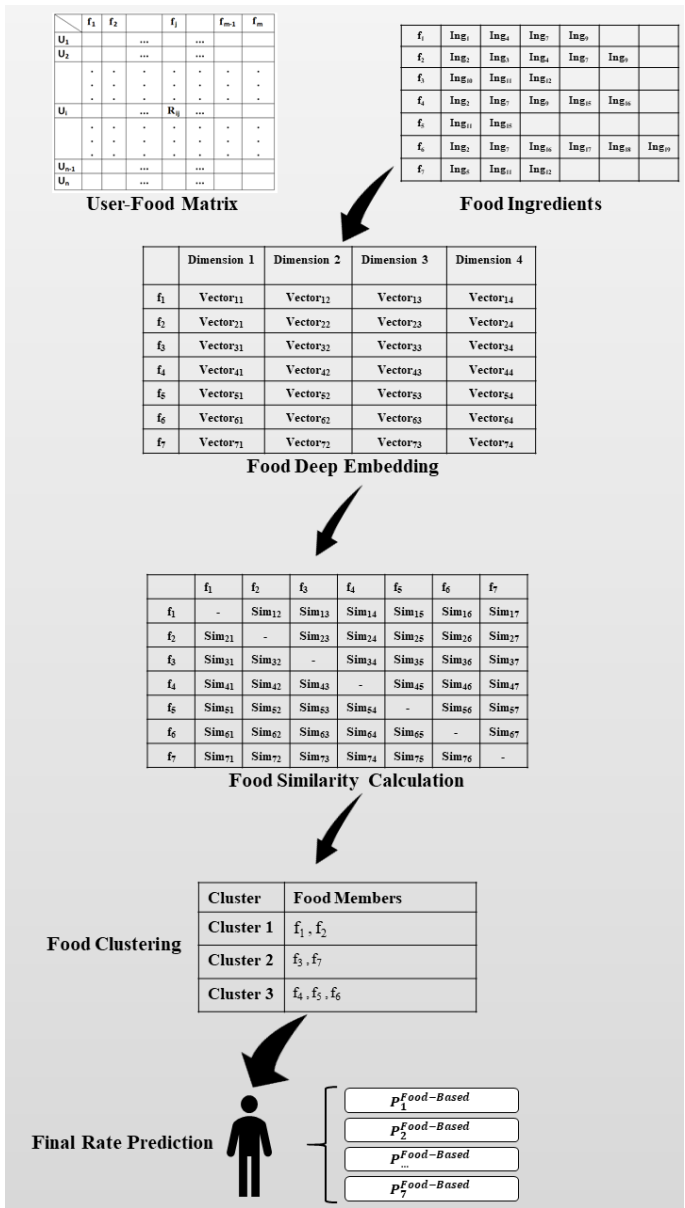
\includegraphics[scale=0.80]{overall_schema_food_based_rating_prediction.png}
    \caption{Food-based rating prediction model for sample dataset with seven users}
    \label{fig:Food-based rating prediction model}
\end{figure}


\section{Top-N Recommendation}
After performing both user-based rating prediction and food-based rating prediction, the final prediction of food $f_i$ for a user $u$ is calculated as a convex combination of these predicted values\cite*{9775081, oulu_tdlgc}. It is done by using the formula:
\begin{equation*}
    p_{i}\left({u}\right)=\beta p_{i}^{u-based}+\left({1-\beta }\right) p_{i}^{f-based}. \tag{7}
\end{equation*}
where $p_i^{u-based}$(u) and $p_i^{f-based}$(u) denotes user-based prediction and food-based prediction on food $f_i$ for user $u$, respectively\cite*{9775081, oulu_tdlgc}. Parameter $\beta$ controls whether user-based or food-based prediction value has a higher priority in final outcome. A higher value of $\beta$ means user-based rating prediction was given a higher priority in influencing the final outcome, while a lower value means food-based rating prediction was given higher priority.